% !TEX program = xelatex
% 编译：E:\tools\tectonic\tectonic.exe -X compile main.tex   （Tectonic 内置 XeTeX + ctex + Fandol）
\documentclass[UTF8, a4paper, 11pt]{ctexart}

\usepackage{amsmath, amssymb}
\usepackage{booktabs}
\usepackage{graphicx}
\usepackage{geometry}
\usepackage{caption}
\usepackage{array}
\usepackage{multirow}
\usepackage{xcolor}
\usepackage[colorlinks=true, linkcolor=blue!55!black, citecolor=blue!55!black,
            urlcolor=blue!55!black]{hyperref}

\geometry{left=2.4cm, right=2.4cm, top=2.6cm, bottom=2.5cm}
\graphicspath{{figures/}}
\captionsetup{font=small, labelfont=bf}
\captionsetup[table]{skip=4pt}
\renewcommand{\arraystretch}{1.08}

\newcommand{\hv}{\mathrm{HV}}
\newcommand{\imwr}{I_{\mathrm{mwr}}}
\newcommand{\imix}{I_{\mathrm{mix3}}}
\newcommand{\irand}{I_{\mathrm{rand}}}
\newcommand{\lam}{\lambda_0}

\title{\bfseries RMOEA/D 求解双目标模糊柔性作业车间调度\\[3pt]
\large ——复现、评价口径纠正与组件有效性再评估}

\author{}
\date{\today}

\begin{document}
% 正文引用的每个数字都由 scripts/paper_export.py 从 logs/ 现场导出为宏。
% 正文只写宏名——正文与表格读同一份数据，数字物理上无法漂移（缺陷 30）。
% 放在 \begin{document} 之后：宏体里有中文（结论句），preamble 里放中文字符串
% 会让 XeTeX 报 "Missing \begin{document}"（实测）。
% 本文件由 scripts/paper_export.py 现场生成，请勿手改。
% 正文引用宏名而非字面数字：数字只有一个来源（缺陷 30）。
\newcommand{\HKready}{1}
\newcommand{\HKn}{66}
\newcommand{\HKthr}{-1.0}
\newcommand{\HKgain}{10}
\newcommand{\HKtp}{3}
\newcommand{\HKfp}{13}
\newcommand{\HKfn}{7}
\newcommand{\HKtn}{43}
\newcommand{\HKaccHold}{0.70}
\newcommand{\HKaccDev}{1.00}
\newcommand{\HKlamLo}{-5.8}
\newcommand{\HKlamHi}{+0.6}
\newcommand{\HKholdPosN}{10}
\newcommand{\HKholdPosLamLo}{-3.98}
\newcommand{\HKholdPosLamHi}{-0.59}
\newcommand{\HKnearBand}{0.5}
\newcommand{\HKnearHalf}{15}
\newcommand{\HKaccRejectAll}{0.85}
\newcommand{\HKaccLiftAbs}{0.152}
\newcommand{\HKpassN}{16}
\newcommand{\HKpassPrec}{0.19}
\newcommand{\HKrecall}{0.30}
\newcommand{\HKverdict}{留出集上净增量显著为正的实例为 10/66（15.2\%），门控命中 3、误放 13、漏放 7，判对率 \HKaccHold。但留出集本身只有 15.2\% 的实例真赚，\textbf{一律拒绝}的判对率就有 \HKaccRejectAll —— 门控比它低 \HKaccLiftAbs，而门控放行的 \HKpassN 个实例里只有 3 个真赚（精确率 \HKpassPrec）。换言之，在这个分布上探针的判别力\textbf{低于不做任何判别}。 其中 15 个实例的 $\lam$ 落在门限 $\pm\HKnearBand$ 个百分点内——这一带在开发集上已被证明即使 30 seeds 也判不稳（\S\ref{sec:seedvar}），故判对率要连同它一起读。}
\newcommand{\TgtAN}{10}
\newcommand{\TgtAPosN}{10}
\newcommand{\TgtASigN}{8}
\newcommand{\TgtARange}{+0.05\% 至 +8.69\%}
\newcommand{\TgtBSigN}{3}
\newcommand{\TgtBSigRange}{+0.54\% 至 +0.73\%}
\newcommand{\TgtBNonSigN}{7}
\newcommand{\TgtBNonSigRange}{-0.22\% 至 +0.02\%}
\newcommand{\TgtBNonSigPMin}{0.17}
\newcommand{\BonfFamN}{8}
\newcommand{\BonfThr}{0.00625}
\newcommand{\SurfInitTenA}{0.024}
\newcommand{\SurfInitEndA}{0.0010}
\newcommand{\SurfInitTenB}{0.064}
\newcommand{\SurfInitEndB}{0.0028}
\newcommand{\SurfInitTenC}{0.091}
\newcommand{\SurfInitEndC}{0.0085}
\newcommand{\SurfDecayLo}{10.7}
\newcommand{\SurfDecayHi}{23.8}
\newcommand{\SurfNonInitMax}{$1.1\times10^{-3}$}
\newcommand{\SurfNonInitArg}{Mk09 的 RL 选算子}
\newcommand{\LadderMixRel}{+3.406}
\newcommand{\LadderMixWins}{10/10}
\newcommand{\LadderMixP}{0.002}
\newcommand{\LadderVnsRel}{+0.421}
\newcommand{\LadderVnsWins}{10/10}
\newcommand{\LadderVnsP}{0.002}
\newcommand{\LadderQpasRel}{+0.030}
\newcommand{\LadderQpasWins}{5/10}
\newcommand{\LadderQpasP}{0.625}
\newcommand{\LadderEliteRel}{+0.082}
\newcommand{\LadderEliteWins}{10/10}
\newcommand{\LadderEliteP}{0.002}
\newcommand{\LadderRlRel}{-0.003}
\newcommand{\LadderRlWins}{6/10}
\newcommand{\LadderRlP}{0.625}
\newcommand{\ProbeRho}{+0.77}
\newcommand{\ProbeRhoP}{0.009}
\newcommand{\FamRho}{+0.83}
\newcommand{\FamP}{0.003}
\newcommand{\PermP}{0.035}
\newcommand{\NullPct}{0.81}
\newcommand{\FamArgmax}{probe_mean_mc_lever_pct}
\newcommand{\HKdevPosN}{3}
\newcommand{\HKdevPosLamLo}{-0.53}
\newcommand{\HKdevPosLamHi}{+0.64}
\newcommand{\HKdevOthLamMax}{-1.06}
\newcommand{\HKdevGap}{0.5}
\newcommand{\PSsdOne}{0.62}
\newcommand{\PSagreeOne}{0.95}
\newcommand{\PSagreeMinOne}{0.50}
\newcommand{\PSmkNineLam}{-1.06}
\newcommand{\PSmkNineAgreeTen}{0.73}
\newcommand{\PSmkNineMargin}{0.06}
\newcommand{\PSn}{10}
\newcommand{\MsRho}{+0.95}
\newcommand{\MsRhoP}{0.0000}
\newcommand{\CalibFamN}{8}
\newcommand{\CalibFamNullPct}{0.81}
\newcommand{\BoxNoSigN}{7}
\newcommand{\BoxNoSigLo}{-0.58}
\newcommand{\BoxNoSigHi}{+0.95}
\newcommand{\BoxNoSigMed}{+0.29}
\newcommand{\BoxNoSigFlipN}{3}
\newcommand{\BndMinLoWl}{136}
\newcommand{\BndMaxLoWl}{2453}
\newcommand{\BndWlSpan}{18.1}
\newcommand{\BndMsSpan}{8.5}
\newcommand{\CalibCells}{50}
\newcommand{\CalibRhoLog}{-0.37}
\newcommand{\CalibRhoLogP}{0.009}
\newcommand{\CalibRhoRaw}{-0.25}
\newcommand{\CalibRhoRawP}{0.076}
\newcommand{\CalibAmpAbsMin}{0.31}
\newcommand{\CalibAmpMax}{47.9}
\newcommand{\CalibAmpLo}{4.9}
\newcommand{\CalibAmpHi}{29.7}
\newcommand{\CalibAmpMix}{5.9}
\newcommand{\CalibAmpQpas}{10.6}
\newcommand{\CalibWorstPair}{RMOEAD|D5}
\newcommand{\CalibSmallThr}{0.02}
\newcommand{\CalibSmallN}{9}
\newcommand{\CalibSmallMed}{16.7}
\newcommand{\CalibRestN}{41}
\newcommand{\CalibRestMed}{7.9}
\newcommand{\CalMkTenQpasInst}{-0.017}
\newcommand{\CalMkTenQpasBox}{-0.829}
\newcommand{\SetNp}{100}
\newcommand{\SetG}{200}
\newcommand{\SetGMax}{2000}
\newcommand{\SetSeeds}{30}
\newcommand{\SetRefLo}{1.02}
\newcommand{\SigLevel}{0.05}
\newcommand{\PctBase}{100}
\newcommand{\PermSubsets}{2000}
\newcommand{\SurfBudgets}{$10\%,25\%,50\%,75\%,100\%$}
\newcommand{\SurfFirstBudget}{10}
\newcommand{\DevN}{10}
\newcommand{\SeedRange}{42--71}
\newcommand{\RunN}{300}
\newcommand{\AnytimeTenXPct}{+1.43}
\newcommand{\AnytimeTenX}{10}
\newcommand{\TscanGapPct}{+0.128}
\newcommand{\TscanGapP}{0.073}
\newcommand{\TscanDz}{+0.37}
\newcommand{\TscanWins}{19/30}
\newcommand{\TscanSpaceGlobal}{1}
\newcommand{\TscanBestTag}{T15}
\newcommand{\TscanNote}{空间内那个最优的 $T$ 同时就是全部 6 档候选中的最优——动作空间没有漏掉任何有意义的东西，}

\maketitle
\thispagestyle{empty}

\begin{abstract}
\noindent
Li 等（2022）提出的 RMOEA/D 用 Q-learning 同时驱动参数自适应（Q-PAS）与变邻域
算子选择（RVNS），在双目标模糊柔性作业车间调度上报告了良好效果。本文在
Brandimarte Mk01--Mk10 上对该算法做了可复现的重实现，并在统一评价口径下重新审计
其每个组件。工作有三点。其一，\textbf{评价口径}：我们指出文献与复现中普遍使用的
"按参与比较的前沿取归一化边界"（下称盒口径）有两个不可修复的缺陷——边界随实例集
与臂集漂移，且系统性放大效应量；实测同一批数据下按臂对汇总的放大为
$\CalibAmpLo\times$ 至 $\CalibAmpHi\times$、\textbf{逐格子最高 $\CalibAmpMax\times$}，
\textbf{倍数并非常数}，更严重的是它会改变现象的形状（把"少数实例显著、
其余与 0 不可区分"抹成"处处微小为正"）。因此本文主张改用由实例数据确定性推出的
\textbf{实例边界口径}，并给出可复现的对照证据。其二，\textbf{组件有效性的重新判定}：
在实例边界口径下，六个阶梯臂的逐级增量为 MIX3 初始化 $\LadderMixRel\%$（\LadderMixWins\ 实例胜出）、
随机 VNS $\LadderVnsRel\%$、精英档案 $\LadderEliteRel\%$，而 Q-PAS 仅 $\LadderQpasRel\%$（$p=\LadderQpasP$，不显著）、
RL 选算子 $\LadderRlRel\%$；进一步用 anytime 轨迹证明算力在 $G=200$ 附近已接近饱和，
因此 RL 组件的失效不是"学不到"，而是\textbf{没有空间可学}。其三，\textbf{可事前判定
的增益}：我们提出一个零代探针——只调用一次初始种群构造（不做任何搜索），
用初始前沿 HV 的杠杆 $\lam$ 预测"某个新实例上 MWR 初始化相对论文口径是否真有净增益"，
并在 66 个 Hurink $e$-data 实例上做完全预注册的留出验证。
\textbf{该门控没有通过这次检验}：它在开发集上与净增益完全分离，在留出集上的判对率
却低于“一律拒绝”这条平凡基线，放行实例的精确率仅 $\HKpassPrec$。
我们据此把“廉价零代门控可以跨分布移植”这个常见默认写成明确的负结果。

\vspace{4pt}
\noindent\textbf{关键词：} 柔性作业车间调度；分解型多目标进化算法；模糊加工时间；
强化学习；消融实验；评价口径；可复现性
\end{abstract}

%======================================================================
\section{引言}
%======================================================================

双目标模糊柔性作业车间调度问题（bi-objective fuzzy flexible job-shop scheduling
problem, FFJSP）要在不确定加工时间下同时最小化最大完工时间与机器总负载，是典型的
NP 难组合优化问题。Li 等\cite{li2022rmoead} 提出的 RMOEA/D 把 Q-learning 同时接在
两个决策点上：一是每代选择 Tchebycheff 分解中的参数 $T$（Q-PAS），二是选择变邻域
搜索的算子（RVNS），并在 Brandimarte 基准上报告了相对基线的改进。

复现这类"学习型元启发式"时，有两个容易出错、且出错方式很隐蔽的地方：

\textbf{(1) 多目标指标的评价口径。} 超体积（HV）需要把两个目标归一化到同一量纲。
把归一化边界取为"参与比较的前沿的极值"（盒口径）是一行代码就能写出的做法，
但它使边界成为一个\textbf{依赖于臂集与实例集}的量：同一份数据，只要换掉比较对象，
HV 读数就变。这在复现里意味着一个组件"有没有效果"的结论会随同批实验的设计而漂移。

\textbf{(2) 比较基准与问题的不对齐。} 当要回答"该不该用我们提出的初始化"时，
正确的对照是\textbf{论文自己的初始化}；而"随机初始化"只能回答"有个好起点值多少"。
这两个量在同一批数据上都算得出来，但用前者去论证后者是无效的。

本文把这两点作为方法学主线，并在严格执行它们之后重新评估 RMOEA/D 的每个组件。
结论是负面的：真正有效的只有初始化与算力总量，两个 RL 组件在本基准上没有可实现空间。
但我们并不止步于负结果——我们进一步给出一个\textbf{零代探针}，它能以一次初始种群
构造的代价事前判定"初始化的净增益在某个新实例上是否会出现"，并在一个 66 实例的
独立留出集上做预注册验证。\textbf{探针没有通过}：跨到 Hurink $e$-data 之后，
它的判别力低于“一律拒绝”这条平凡基线。我们把这个失败也完整报告出来 ——
它正是本文方法学主张的自我检验：门限若只在挑出它的那批实例上成立，就不能算门控。

\paragraph{贡献。}
\begin{itemize}\itemsep2pt
  \item 量化了盒口径的偏差：同一批数据、同一臂对，效应量被放大约一个数量级，
        且\textbf{放大倍数不是常数}（按臂对汇总 $\CalibAmpLo\times$--$\CalibAmpHi\times$，
        逐格子最高 $\CalibAmpMax\times$），
        显著性检验的 $p$ 与胜出场数同样改变（\S\ref{sec:caliber}）。
  \item 在实例边界口径下重新给出六臂消融阶梯的逐级效应，并把"算力饱和"量化，
        由此把 RL 组件的失效解释为\textbf{动作空间与算力上都没有空间}（\S\ref{sec:res}）。
  \item 提出零代探针门控（$\lam$ = 初始前沿 HV 杠杆）：它在开发集上与净增益完全分离，
        但在 66 实例的预注册留出集上\textbf{没有通过}——判对率 $\HKaccHold$ 低于
        “一律拒绝”的平凡基线 $\HKaccRejectAll$，放行实例的精确率仅 $\HKpassPrec$，
        召回仅 $\HKrecall$（\S\ref{sec:hurink}）；此外回答"门控需要多少 seed"（\S\ref{sec:seedvar}）。
  \item 全部脚本、原始日志与"一个数字一个来源"的导出流程随文公开，
        论文中每个数字都由 \texttt{scripts/paper\_export.py} 从 \texttt{logs/} 现场生成。
\end{itemize}

%======================================================================
\section{问题、算法与指标}
%======================================================================

\subsection{双目标模糊 FJSP}
给定 $n$ 个工件、$m$ 台机器，每个工件的每道工序的加工时间用三角模糊数
$\tilde t=(t_1,t_2,t_3)$ 表示，且可在其可行机器集合中任选一台加工。目标是
\begin{equation}
  \min \; F = \bigl( f_1 = C_{\max},\; f_2 = W \bigr),
\end{equation}
其中 $C_{\max}$ 为最大完工时间，$W$ 为机器总负载。三角模糊数的比较与
"模糊$\to$确定"（crisp）折算沿用 Li 等\cite{li2022rmoead} 的约定，
以保证与本项目复现对象一致；模糊区间由实例名与随机种子共同决定，
因此同一实例在不同 seed 下的模糊时间不同，这使"同 seed 配对"成为
一切组间比较的基本单位。

\subsection{超体积（HV）}
本文的单一汇总指标是前沿的 HV，参考点固定为 $\mathrm{ref}=(1.02,1.02)$。
HV 的\textbf{归一化边界}取法有两种，本文的全部结论都建立在第二种之上
（\S\ref{sec:caliber}）：
\begin{itemize}\itemsep1pt
  \item \textbf{实例边界口径}（本文采用）：边界 $(\mathrm{lo},\mathrm{hi})$ 由
        实例数据确定性推出（下界取临界路径下界、上界取全部工序最长时间之和），
        \textbf{与参与比较的臂集无关}。实现见 \texttt{instance\_hv\_bounds()}，
        算法落盘的 \texttt{final\_hv} 用的就是它。
  \item \textbf{盒口径}（仅作对照）：边界取参与比较的\textbf{前沿的极值}，
        实现见 \texttt{estimate\_hv\_bounds()}。
\end{itemize}

\subsection{RMOEA/D 的可插拔组件}
复现中我们把算法拆成六个臂（表~\ref{tab:ladder} 的"阶梯"列），每一级相对上一级
只打开一个组件：
$D_1$ 为纯 MOEA/D（固定 $T=10$，关闭 MIX3/RVNS/Q-PAS/精英档案）；
$D_2$ 打开 MIX3 初始化；$D_3$ 打开随机 VNS；$D_4$ 把固定的 $T$ 换成 Q-PAS；
$D_5$ 打开精英档案；\textsf{RMOEAD} 把随机 VNS 换成 RL 选算子。
这一阶梯与文献\cite{li2022rmoead} 表 5 的步骤分解对齐，因而"每一级是否有效"
就是对该文主张的逐条检验。\textsf{RMOEAD} 与 $D_5$ 只差"谁选算子"，
是检验 RL 组件\textbf{最干净的单变量对照}（等算力、同其它一切）。

%======================================================================
\section{评价口径：一个会改变结论的隐藏变量}\label{sec:caliber}
%======================================================================

\subsection{盒口径的两个缺陷}
\textbf{(a) 跨实例污染。} 若把多个实例的前沿并进同一个盒，边界会跨越相差一个
数量级的实例（如 Mk07 的 HV 量级约 $150/700$、Mk10 约 $300/2000$），
于是所有实例的值都被"拉"到相近区间，读出"所有变体都近乎完美"的假象。
凡按 $(\text{臂},\text{seed})$ 在多个实例上摊平再取极值的写法都会踩这一点。

\textbf{(b) 臂集污染。} 盒只应包含\textbf{参与比较的臂}。若把与本次比较无关的臂
一并放进盒（例如把另做的一批 $T$ 扫描臂混进消融实验的日志），上界被无关数据撑高，
同一份数据的所有读数随之改变。本文的对照实验因此\textbf{逐臂对}重算边界，
即盒内恰好只有被比较的两个臂。

\subsection{量化的后果}
表~\ref{tab:ladder} 右三列给出同一批数据（8 臂 $\times$ 10 实例 $\times$ 30 seeds）
在两种口径下的读数。三点值得注意：

\begin{enumerate}\itemsep2pt
  \item \textbf{放大倍数不是常数}：按臂对汇总（比值之比，\S\ref{sec:stat}）从
        $\CalibAmpLo\times$ 到 $\CalibAmpHi\times$ 不等，
        逐格子最高达 $\CalibAmpMax\times$（Mk10 的 $D_4|D_3$：实例边界 $\CalMkTenQpasInst\%$
        $\to$ 盒口径 $\CalMkTenQpasBox\%$）。因此"盒口径数字除以固定倍数即可折回"是错的。
        图~\ref{fig:ladder} 把两种口径并排画出，$D_2|D_1$ 的相对增幅被放大
        $\CalibAmpMix\times$，而几乎为零的 $D_4|D_3$ 被放大 $\CalibAmpQpas\times$
        ——\textbf{越接近零的效应，相对放大越厉害}：$\CalibCells$ 个（实例，臂对）
        格子里，$|\Delta \hv|\le 0.02\%$（"接近零"的显式阈值）的 $\CalibSmallN$ 个
        格子放大中位数为 $\CalibSmallMed\times$，其余 $\CalibRestN$ 个只有
        $\CalibRestMed\times$。
        \textbf{秩相关的口径必须写明}：对 $\log_{10}|\text{放大}|$ 取秩得
        $\mathrm{Spearman}=\CalibRhoLog$（$p=\CalibRhoLogP$）；若直接对原始放大倍数
        取秩则只有 $\CalibRhoRaw$（$p=\CalibRhoRawP$，未过线）。
        两者方向一致、强弱不同——不写出取对数这一步，读者无法复核这个数。
        这正是本文主张的"\textbf{任何数字离开其口径不可引用}"的一个具体例子。
  \item \textbf{$p$ 值与胜出场数也会变}。这一点比幅度更容易被忽略：口径改变
        不只是"数字大小"，而是\textbf{显著性判定本身}。
  \item \textbf{现象的形状会变}。本文 \S\ref{sec:twoTargets} 会遇到一个
        "3/10 实例显著、7/10 与 0 不可区分"的双峰形态；在盒口径下，那 7 个
        非显著实例变成从 $\BoxNoSigLo\%$ 散到 $\BoxNoSigHi\%$ 的一团
        （中位 $\BoxNoSigMed\%$，且其中 $\BoxNoSigFlipN$ 个\textbf{翻转了符号}），
        于是被读成"效应弱但普遍存在"。\textbf{形状的失真比幅度的失真更难察觉}。
\end{enumerate}

\subsection{报数规则}
本文后续一律遵守：\textbf{效应量与显著性只报实例边界口径}；对照展示盒口径时必须
同时给出放大倍数；任何数字离开其口径不可引用；跨实例只比\textbf{相对差与秩}，
不比 HV 绝对值（各实例边界不同）。

%======================================================================
\section{实验设置}
%======================================================================

\subsection{实例集}
表~\ref{tab:instances} 列出实例。开发集为 Brandimarte Mk01--Mk10（论文原始基准），
用于复现与门限标定；留出集为\textbf{Hurink $e$-data 的全部 66 个实例}，
用于留出验证。留出集的选择完全预注册：取该数据集的全部实例，不做任何按结果的挑选；
实例文件取自公开基准库并以 SHA-256 记录来源（\texttt{data/hurink/PROVENANCE.json}）。

\begin{table}[t]
  \centering
  \caption{实例集特征：(a) 开发集 Brandimarte Mk01--Mk10（只占左栏）；(b) 留出集 Hurink $e$-data，按 (工件, 机器, 工序) 分组合并后续排为左右两栏}
  \label{tab:instances}
  \footnotesize
  {\setlength{\tabcolsep}{4pt}%
  \begin{tabular}{lrrrrr@{\hspace{10pt}}lrrrrr}
    \toprule
    \multicolumn{12}{l}{\textit{(a) Brandimarte Mk01--Mk10：复现与消融的开发集}}\\
    \cmidrule(lr){1-12}
    \textit{实例} & \textit{工件} & \textit{机器} & \textit{工序} & \textit{弹性比} & \textit{$c_v$} & \textit{实例} & \textit{工件} & \textit{机器} & \textit{工序} & \textit{弹性比} & \textit{$c_v$} \\
    \midrule
    Mk01 & 10 & 6 & 55 & 2.09 & 0.56 &  &  &  &  &  &  \\
    Mk02 & 10 & 6 & 58 & 4.10 & 0.50 &  &  &  &  &  &  \\
    Mk03 & 15 & 8 & 150 & 3.01 & 0.63 &  &  &  &  &  &  \\
    Mk04 & 15 & 8 & 90 & 1.91 & 0.63 &  &  &  &  &  &  \\
    Mk05 & 15 & 4 & 106 & 1.71 & 0.32 &  &  &  &  &  &  \\
    Mk06 & 10 & 10 & 150 & 3.27 & 0.63 &  &  &  &  &  &  \\
    Mk07 & 20 & 5 & 100 & 2.83 & 0.64 &  &  &  &  &  &  \\
    Mk08 & 20 & 10 & 225 & 1.43 & 0.48 &  &  &  &  &  &  \\
    Mk09 & 20 & 10 & 240 & 2.52 & 0.43 &  &  &  &  &  &  \\
    Mk10 & 20 & 15 & 240 & 2.98 & 0.47 &  &  &  &  &  &  \\
    \midrule
    \multicolumn{12}{l}{\textit{(b) Hurink $e$-data：66 个实例，全部用作\textbf{独立留出集}（不挑选）}}\\
    \cmidrule(lr){1-12}
    \textit{实例数} & \textit{工件} & \textit{机器} & \textit{工序} & \textit{弹性比} & \textit{} & \textit{实例数} & \textit{工件} & \textit{机器} & \textit{工序} & \textit{弹性比} & \textit{} \\
    $\times$1 & 6 & 6 & 36 & 1.17 & & $\times$4 & 20 & 5 & 100 & 1.13 & \\
    $\times$1 & 7 & 7 & 49 & 1.18 & & $\times$2 & 20 & 5 & 100 & 1.14 & \\
    $\times$3 & 10 & 5 & 50 & 1.20 & & $\times$9 & 10 & 10 & 100 & 1.14 & \\
    $\times$2 & 10 & 5 & 50 & 1.18 & & $\times$2 & 15 & 10 & 150 & 1.15 & \\
    $\times$1 & 13 & 4 & 52 & 1.21 & & $\times$1 & 15 & 10 & 150 & 1.14 & \\
    $\times$1 & 11 & 5 & 55 & 1.20 & & $\times$2 & 15 & 10 & 150 & 1.16 & \\
    $\times$1 & 14 & 4 & 56 & 1.20 & & $\times$4 & 20 & 10 & 200 & 1.14 & \\
    $\times$1 & 12 & 5 & 60 & 1.18 & & $\times$1 & 20 & 10 & 200 & 1.13 & \\
    $\times$1 & 10 & 6 & 60 & 1.17 & & $\times$3 & 15 & 15 & 225 & 1.15 & \\
    $\times$1 & 8 & 8 & 64 & 1.17 & & $\times$2 & 15 & 15 & 225 & 1.14 & \\
    $\times$1 & 8 & 9 & 72 & 1.17 & & $\times$2 & 30 & 10 & 300 & 1.14 & \\
    $\times$4 & 15 & 5 & 75 & 1.15 & & $\times$3 & 30 & 10 & 300 & 1.13 & \\
    $\times$1 & 15 & 5 & 75 & 1.16 & & $\times$2 & 20 & 15 & 300 & 1.13 & \\
    $\times$1 & 10 & 10 & 99 & 1.13 & & $\times$1 & 20 & 15 & 300 & 1.13 & \\
    $\times$8 & 10 & 10 & 100 & 1.13 & &  &  &  &  &  &  \\
    \bottomrule
  \end{tabular}
  }
  \par\vspace{3pt}\footnotesize\begin{minipage}{\linewidth}弹性比 = 每道工序可选机器数的均值；$c_v$ = 模糊三角加工时间的变异系数。Mk01--Mk10 用于复现、消融与\textbf{门限标定}。Hurink $e$-data 共 66 个实例，规模 36--300 道工序；(b) 段左右两栏续排，按 (工件, 机器, 工序) 分组合并，$\times c$ 为组内实例数。全部实例都进留出集，\textbf{没有任何按结果的事后挑选}。\end{minipage}
\end{table}


\subsection{参数与算力}
种群规模 $N_p=100$，代数 $G=200$，每个配置 30 个随机种子（42--71），
$\mathrm{ref}=(1.02,1.02)$。所有组间比较都做\textbf{同 seed 配对}，
以消掉"模糊时间随 seed 变"带来的实例内噪声。响应面实验（\S\ref{sec:surface}）
另在 $G=2000$ 上限下按墙钟预算分档，用于观察"算力变大时效应如何变"。

\subsection{统计口径}\label{sec:stat}
同一组比较给两套读数：\textbf{实例级}（先在实例内对 30 个 seed 取均值，$n=10$ 或
$n=66$）与 \textbf{run 级}（逐 seed 配对，$n=300$）。检验用 Wilcoxon 符号秩，
效应量用配对 Cohen's $d_z$；相对增幅定义为
$\overline{\Delta \hv}/\overline{\hv}_{\text{上一级}}$（先求均值再作比，
不用 $\overline{\Delta/\hv}$——后者在效应$\approx 0$ 时会反号；\textbf{盒口径的
放大倍数也用同一约定}：$\overline{\Delta \hv}_{\text{盒}}/\overline{\Delta \hv}_{\text{实例}}$，
而不是逐 run 放大倍数的平均，两者相差可达数倍）。
存在多个候选预测变量时，用\textbf{置换零假设}（固定预测变量的秩矩阵、
只打乱实例与目标的对应）做家族错误率校正，而不是 Bonferroni：
在 $n=10$、\CalibFamN 个候选的设定下，纯噪声的 $\max|\rho|$ 的 95\% 分位就有
$\CalibFamNullPct$，
Bonferroni 的 $\BonfThr$ 门槛过松。

\subsection{复现环境}
代码为 Python 实现，数值依赖 NumPy/SciPy；实验按实例分批驱动并支持断点续跑。
论文的每一个数字都由 \texttt{scripts/paper\_export.py} 从结果文件现场生成，
取不到即报错，不允许人工填数。

%======================================================================
\section{结果}\label{sec:res}
%======================================================================

\subsection{组件阶梯：只有初始化与随机 VNS 站得住}
表~\ref{tab:ladder} 与图~\ref{fig:ladder} 给出六臂阶梯的逐级增量。
在实例边界口径下：MIX3 初始化 $\LadderMixRel\%$（\LadderMixWins\ 实例胜出，
$p=\LadderMixP$）、随机 VNS $\LadderVnsRel\%$（\LadderVnsWins，$p=\LadderVnsP$）、
精英档案 $\LadderEliteRel\%$（\LadderEliteWins，$p=\LadderEliteP$）；
而 Q-PAS 只有 $\LadderQpasRel\%$（\LadderQpasWins，$p=\LadderQpasP$，不显著），
RL 选算子 $\LadderRlRel\%$（\LadderRlWins，不显著）。
注意最后一行的含义：\textsf{RMOEAD} 与 $D_5$ 的唯一差别是"用 RL 选算子"还是
"随机选算子"，等算力、同其它一切——\textbf{把 RL 组件换成随机选择，结果没有区别}。

\begin{table}[htbp]
  \centering
  \caption{组件阶梯的逐级增量：实例边界口径（正文引用）与盒口径（仅作对照）}
  \label{tab:ladder}
  \footnotesize
  {\setlength{\tabcolsep}{4.5pt}%
  \begin{tabular}{llrrlrrr}
    \toprule
    \multicolumn{6}{c}{\textbf{实例边界口径}} & \multicolumn{2}{c}{\textbf{盒口径}} \\
    \cmidrule(lr){1-6}\cmidrule(lr){7-8}
    阶梯 & 组件 & $\Delta$HV 相对增幅(\%) & 实例胜出 & $d_z$ & $p$ & 相对增幅(\%) & 放大 \\
    \midrule
    D2$|$D1 & MIX3 初始化 & +3.406 & 10/10 & +0.98 & $2.0\times 10^{-3}{}^{**}$ & +19.956 & 5.9$\times$ \\
    D3$|$D2 & 随机 VNS & +0.421 & 10/10 & +0.61 & $2.0\times 10^{-3}{}^{**}$ & +4.199 & 10.0$\times$ \\
    D4$|$D3 & Q-PAS & +0.030 & 5/10 & +0.05 & $0.625$ & +0.314 & 10.6$\times$ \\
    D5$|$D4 & 精英档案 & +0.082 & 10/10 & +0.65 & $2.0\times 10^{-3}{}^{**}$ & +0.400 & 4.9$\times$ \\
    RMOEAD$|$D5 & RL 选算子 & -0.003 & 6/10 & -0.01 & $0.625$ & -0.091 & 29.7$\times$ \\
    \bottomrule
  \end{tabular}
  }
  \par\vspace{3pt}\footnotesize\begin{minipage}{\linewidth}Mk01--Mk10，每格 $n=30$ seeds 同 seed 配对。$\Delta$HV 相对增幅为\textbf{逐实例} $\overline{\Delta\mathrm{HV}}/\overline{\mathrm{HV}}_{\text{上一级}}$ 的跨实例均值（不用 $\overline{\Delta/\mathrm{HV}}$：效应$\approx 0$ 时会反号）。$d_z$ 为 run 级池化配对效应量（$n=300$），$p$ 为实例级 Wilcoxon（$n=10$）。盒口径一列是\textbf{同一批数据}换口径重算的结果，用来量化口径的影响；正文的效应量一律取实例边界口径。\end{minipage}
\end{table}


\begin{figure}[t]
  \centering
  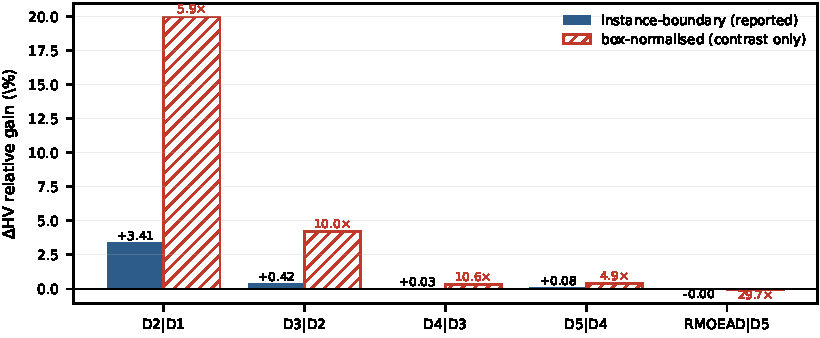
\includegraphics[width=0.86\linewidth]{fig_ladder.pdf}
  \caption{六臂阶梯的逐级 $\Delta$HV 相对增幅：实例边界口径（实心，正文引用）
  与盒口径（斜纹，仅作对照）。盒口径把接近零的效应相对放大得最多，
  红色标注为放大倍数。}
  \label{fig:ladder}
\end{figure}

\subsection{算力–算法响应面：不是学不到，是没空间可学}\label{sec:surface}
图~\ref{fig:surface} 把每个臂对放在同一族"墙钟预算分数"
（$10\%,25\%,50\%,75\%,100\%$，$G$ 上限 2000）上比较。
初始化的效应随算力增加而\textbf{显著衰减}：在 $10\%$ 预算处三个实例的
$|\Delta \hv|$ 为 $\SurfInitTenA/\SurfInitTenB/\SurfInitTenC$，到全额预算时只剩
$\SurfInitEndA/\SurfInitEndB/\SurfInitEndC$（衰减 $\SurfDecayLo$--$\SurfDecayHi$ 倍）；
而 RL 选算子在\textbf{所有}预算档上都贴着零线。
表~\ref{tab:surface} 给出全额预算下的绝对值：非初始化组件的最大者也只有
\SurfNonInitMax（\SurfNonInitArg）。

\begin{table}[t]
  \centering
  \caption{算力全部花完时（100\% 预算）各组件相对上一级的 $\Delta$HV 绝对值}
  \label{tab:surface}
  \small
  \begin{tabular}{llrrr}
    \toprule
    臂对 & 组件 & Mk07 & Mk09 & Mk10 \\
    \midrule
    D2$|$D1 & MIX3 初始化 & +0.001 & +0.003 & +0.009 \\
    RMOEAD$|$D5 & RL 选算子 & +0.000 & -0.001 & -0.000 \\
    \bottomrule
  \end{tabular}
  \par\vspace{3pt}\footnotesize\begin{minipage}{\linewidth}每列一个实例；预算按\textbf{墙钟}（\texttt{anytime} 轨迹）分五分位（\SurfBudgets，$G$ 上限 \SetGMax）。把算力加到上限以后，除初始化以外的组件增量都不超过 $1.1\times10^{-3}$（最大者为 Mk09 的 RL 选算子，绝对值）。\end{minipage}
\end{table}


\begin{figure}[t]
  \centering
  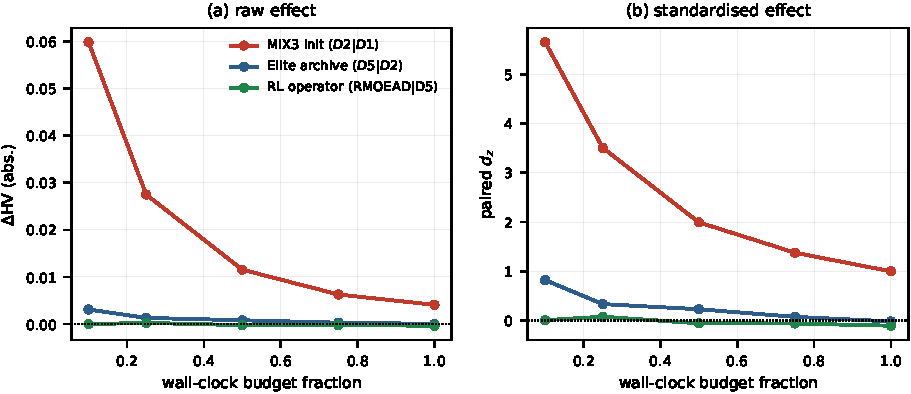
\includegraphics[width=\linewidth]{fig_surface.pdf}
  \caption{算力–算法响应面。(a) 原始 $\Delta$HV 随墙钟预算的衰减；
  (b) 标准化效应 $d_z$。初始化（红）是唯一随算力增加而衰减的显著效应，
  RL 选算子（绿）全程贴零。}
  \label{fig:surface}
\end{figure}

\subsection{同一批数据上的两个目标量}\label{sec:twoTargets}
MWR 是我们的一个派工式工序初始化变体（按剩余工时规则决定工序顺序，
只在 MA 维度保留原算法的随机性）。要问"该不该用它"，必须把对照设成
\textbf{论文自己的 MIX3 初始化}（目标 B）；把它对照随机初始化（目标 A）
回答的是另一个问题。表~\ref{tab:targets} 与图~\ref{fig:targets} 同时给出两者。

\begin{itemize}\itemsep2pt
  \item \textbf{目标 A}（$\imwr$ vs.\ $\irand$）：\TgtAPosN/\TgtAN\ 实例为正、\textbf{\TgtASigN\ 个显著}
        （只有 Mk01 与 Mk05 不显著），幅度 \TgtARange。
        这说明"有个好起点"普遍有价值。
  \item \textbf{目标 B}（$\imwr$ vs.\ $\imix$，净增量）：\textbf{只有 \TgtBSigN/\TgtAN\ 显著}，
        幅度 \TgtBSigRange；\textbf{其余 \TgtBNonSigN\ 个与 0 不可区分}（\TgtBNonSigRange，
        全部不显著）。
\end{itemize}

\noindent 因此 MWR 的净增量是\textbf{全有或全无}的：它在少数实例上有值，
在其余实例上一分不赚。把目标 A 的读数当作目标 B 的答案，正是本文要提醒的
第二类错位；它会把"Mk10 上有净增益"错误地推广为"该初始化普遍更好"。

\begin{table}[htbp]
  \centering
  \caption{同一批数据、两个目标量：目标 A（$I_{\mathrm{mwr}}$ vs.\ $I_{\mathrm{rand}}$）与目标 B（$I_{\mathrm{mwr}}$ vs.\ $I_{\mathrm{mix3}}$）}
  \label{tab:targets}
  \footnotesize
  \begin{tabular}{rrrrrrrr}
    \toprule
    \multicolumn{5}{c}{\textbf{目标 A：有好起点值多少}} & \multicolumn{3}{c}{\textbf{目标 B：MWR 相对论文口径的净增量}} \\
    \cmidrule(lr){1-5}\cmidrule(lr){6-8}
    实例 & $\Delta$HV(\%) & 胜出 & $d_z$ & $p$ & $\Delta$HV(\%) & 胜出 & $p$ \\
    \midrule
    Mk01 & +0.047 & 13/30 & +0.06 & $0.685$ & −0.073 & 15/30 & $0.626$ \\
    Mk02 & +0.525 & 22/30 & +0.74 & $5.5\times 10^{-4}{}^{***}$ & +0.010 & 17/30 & $0.556$ \\
    Mk03 & +3.879 & 30/30 & +3.88 & $<10^{-4}{}^{***}$ & +0.023 & 17/30 & $0.328$ \\
    Mk04 & +0.467 & 21/30 & +0.52 & $0.013{}^{*}$ & −0.224 & 12/30 & $0.171$ \\
    Mk05 & +0.238 & 16/30 & +0.24 & $0.184$ & +0.024 & 15/30 & $1.000$ \\
    Mk06 & +4.871 & 30/30 & +5.76 & $<10^{-4}{}^{***}$ & +0.730 & 29/30 & $<10^{-4}{}^{***}$ \\
    Mk07 & +1.593 & 30/30 & +3.25 & $<10^{-4}{}^{***}$ & −0.009 & 16/30 & $1.000$ \\
    Mk08 & +0.944 & 29/30 & +1.55 & $<10^{-4}{}^{***}$ & +0.542 & 28/30 & $<10^{-4}{}^{***}$ \\
    Mk09 & +6.584 & 30/30 & +5.88 & $<10^{-4}{}^{***}$ & +0.012 & 18/30 & $0.685$ \\
    Mk10 & +8.692 & 30/30 & +8.25 & $<10^{-4}{}^{***}$ & +0.690 & 29/30 & $<10^{-4}{}^{***}$ \\
    \bottomrule
  \end{tabular}
  \par\vspace{3pt}\footnotesize\begin{minipage}{\linewidth}$n=\SetSeeds$ seeds，同 seed 配对；$\Delta$HV 为实例边界口径的相对增幅。目标 A 上 10/10 为正（“好起点”这一级确有普遍收益），但\textbf{目标 B 只有 3/10 显著、其余 7 个与 0 不可区分}（配对 Wilcoxon $p\ge0.17$；注意 $\Delta$HV 并非精确的 0，非显著实例中仍为正的最大者是 $+0.024\%$，故“有增益”必须按显著性而非非零来判）：MWR 的净增量是全有或全无，并非“普遍成立但幅度较小”。拿 A 的结论回答 B 的问题即为目标量错位（缺陷 26）。\end{minipage}
\end{table}


\begin{figure}[t]
  \centering
  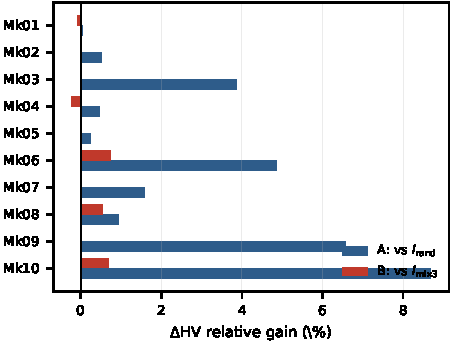
\includegraphics[width=0.52\linewidth]{fig_targets.pdf}
  \caption{两个目标量的逐实例比较。目标 A（蓝）处处为正；
  目标 B（红）只在 Mk06/Mk08/Mk10 上显著为正，其余七个与 0 不可区分。}
  \label{fig:targets}
\end{figure}

\subsection{零代探针：把事后解释升级为事前判据}
既然净增益是"全有或全无"，一个自然的问题是：\textbf{能不能事前知道某个实例属于哪一类？}
最直接的判别量是"初始化的 makespan/HV 杠杆"，但它通常是事后量
（从末代档案算）。我们提出的探针只调用一次初始种群构造（等价于 $G=0$，
一次搜索都不做），取两个变体初始前沿 HV 的比值：
\begin{equation}
  \lam = \frac{\overline{\hv_0}(\imwr) - \overline{\hv_0}(\imix)}
               {\overline{\hv_0}(\imix)} \times 100\%,
\end{equation}
其中 $\overline{\hv_0}$ 为 30 个 seed 的初始前沿 HV 均值（实例边界口径、
ref 同正式实验）。代价是每实例 $\times$ 30 seeds 约 1.4\,s。

在开发集（Mk01--Mk10）上，净增益为正的 \HKdevPosN 个实例的 $\lam$ 都落在
$[\HKdevPosLamLo\%,\HKdevPosLamHi\%]$ 内，其余七个都低于门限 $\HKthr\%$
（最接近的 Mk09 为 $\HKdevOthLamMax\%$）；取门限 $\lam \ge \HKthr\%$ 即
\textbf{完全分离}：\HKdevPosN/\HKdevPosN 命中、0 误放、0 漏放。
该门限在开发集上标定后\textbf{冻结}，不再按留出集调整。

这里必须把两个相关系数\textbf{分开}报，否则会重犯本文所批评的那类错位：
$\lam$ 自身 $\rho=\ProbeRho$（名义 $p=\ProbeRhoP$）；若改取 9 个事前候选的家族最大，
最高者并不是 $\lam$ 而是"初始种群\textbf{平均} makespan 杠杆"，$\rho=\FamRho$、
置换校正 $p=\PermP$。注意家族零假设下 $\max|\rho|$ 的 $95\%$ 分位为 $\NullPct$，
即 \textbf{$\lam$ 自身过不了这道家族校正}（$\ProbeRho<\NullPct$）。
因此我们\textbf{不}以 $\rho$ 的显著性作为门控依据，只以下面的门限分类结果为准；
这也正是必须做独立留出验证的原因。

需要强调的是，事后量"最终 makespan 杠杆"与净增益的相关更高（$\rho=\MsRho$），
但\textbf{用它做门控是循环论证}：要算它必须先把两个臂都跑完。
探针的价值恰恰在于代价只有一次初始种群构造。

%======================================================================
\section{独立留出验证：Hurink $e$-data 的 66 个实例}\label{sec:hurink}
%======================================================================

\ifnum\HKready=0
  \noindent\textbf{（留出验证数据尚未生成：本节数字块、表格与图将在
  \texttt{hurink\_aig.json} 就绪后由导出器自动填充。）}
\fi

\noindent 为什么还需要一个独立留出集：开发集只有 $n=10$，\S\ref{sec:twoTargets}
"3 个显著、7 个与 0 不可区分"这个形态本身就建立在这点样本上，
而门限又是从同一批实例上挑出来的，因此开发集上的"完全分离"不能作为证据。
我们把门限 $\lam\ge\HKthr\%$ 原样搬到留出集——实例是 Hurink $e$-data 的
\textbf{全部 \HKn 个}，不做任何按结果的挑选；每个实例跑 $\imwr$ 与 $\imix$
两个臂、每臂 30 个种子，参数与算力与开发集完全一致。

\HKverdict

\noindent 表~\ref{tab:gate} 给出两个集合上的混淆矩阵，表~\ref{tab:hurink} 逐实例列出
探针 $\lam$ 与目标 B 的净增量。留出集的 $\lam$ 取值范围是
$[\HKlamLo\%,\HKlamHi\%]$，而开发集正例的 $\lam$ 落在
$[\HKdevPosLamLo\%,\HKdevPosLamHi\%]$——两个集合的 $\lam$ 分布并不同构，
这正是"门限在开发集上冻结、再到留出集检验"要暴露的东西：
门控可靠与否，取决于留出集的 $\lam$ 有多少落在门限的决策边界附近。

\noindent \textbf{这个判对率必须与平凡基线并列看，否则容易读反。}留出集上真正有增益的
实例只有 $\HKgain/\HKn$，所以\textbf{不分青红皂白一律拒绝}就能得到 $\HKaccRejectAll$
的判对率，\textbf{比门控的 $\HKaccHold$ 还高 $\HKaccLiftAbs$}。门控一共放行了
$\HKpassN$ 个实例，其中只有 $\HKtp$ 个真赚（精确率 $\HKpassPrec$）；而 $\HKgain$ 个
真赚的实例里有 $\HKfn$ 个被拦下（召回 $\HKrecall$）。也就是说，在这个分布上，
探针的判别\textbf{不如不做判别}。

这个负结果要读准两点。其一，它\textbf{不}说明 MWR 无效——净增量是否普遍存在，由
\S\ref{sec:twoTargets} 的目标 B 回答；它说明的是“\textbf{用一个零代探针事先判断
该不该用它}”这个方案在跨分布时不可靠：门限是在 $n=10$ 的开发集上挑出来的（在那里
它恰好拿到 $\HKaccDev$ 的判对率，把 $10$ 个实例全部判对），而 Hurink 上 $\lam$ 的
分布与开发集并不同构，$[\HKlamLo\%,\HKlamHi\%]$ 的跨度远大于开发集正例所在的
$[\HKdevPosLamLo\%,\HKdevPosLamHi\%]$。其二，判对率里确实有一部分被决策边界吃掉了——
$\HKnearHalf$ 个实例的 $\lam$ 落在门限 $\pm\HKnearBand$ 个百分点内，而 \S\ref{sec:seedvar}
已证明这一带即使 30 个 seed 也判不稳——但\textbf{精确率与召回不受这个解释的庇护}：
即使把所有贴边实例都判对，“门控说可以”的时候仍然有近八成是错的。
所以跨分布的可移植性不是靠调门限能补的。

\begin{table}[t]
  \centering
  \caption{零代门控的混淆矩阵（门限在开发集上标定后冻结：$\lambda_0\ge\HKthr\%$）}
  \label{tab:gate}
  \small
  \begin{tabular}{lrrrrrr}
    \toprule
    集合 & $n$ & 命中 & 误放 & 漏放 & 正确拒绝 & 判对率 \\
    \midrule
    开发集 Mk01--Mk10 & 10 & 3 & 0 & 0 & 7 & 1.00 \\
    留出集 Hurink $e$-data & 66 & 3 & 13 & 7 & 43 & 0.70 \\
    \bottomrule
  \end{tabular}
  \par\vspace{3pt}\footnotesize\begin{minipage}{\linewidth}“命中”= 预测有增益且确实有；“误放”= 预测有而实际为 0；“漏放”= 预测没有而实际有。开发集是门限的标定集，只有留出集一列是无偏的。\end{minipage}
\end{table}

\begin{table}[t]
  \centering
  \caption{独立留出集（Hurink $e$-data）}
  \label{tab:hurink}
  \small
  \begin{tabular}{lll}
    \toprule
    \multicolumn{3}{l}{\textbf{留出验证数据尚未生成}}\\
    \bottomrule
  \end{tabular}
  \par\vspace{3pt}\footnotesize\begin{minipage}{\linewidth}本表为占位：\texttt{logs/hurink\_aig.json} 未就绪。生成后由 \texttt{scripts/paper\_export.py} 覆盖。\end{minipage}
\end{table}


\begin{figure}[t]
  \centering
  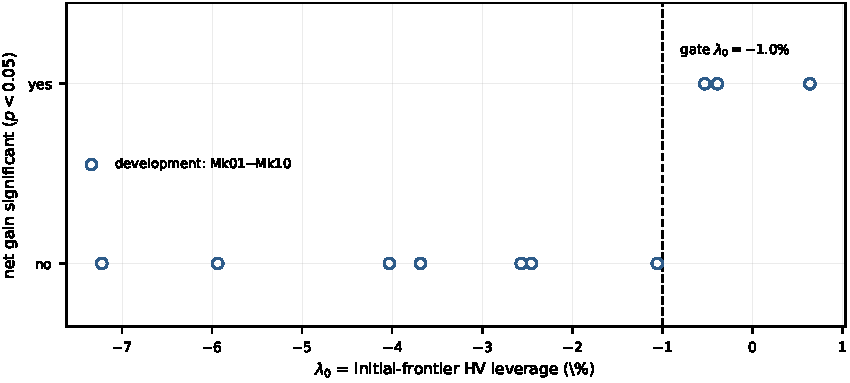
\includegraphics[width=0.86\linewidth]{fig_gate.pdf}
  \caption{零代门控在开发集（圆）与留出集（三角）上的分离情况。
  门限 $\lam=\HKthr\%$ 在开发集上标定后冻结。}
  \label{fig:gate}
\end{figure}

%======================================================================
\section{门控需要几个 seed？}\label{sec:seedvar}
%======================================================================

零代探针虽然便宜，但它仍需要 30 个 seed。开发集上两类实例的 $\lam$ 只相隔约
$\HKdevGap$ 个百分点（正例最低 $\HKdevPosLamLo\%$，非正例最高 $\HKdevOthLamMax\%$），
因此"少采几个 seed 会不会翻掉判定"必须实测，
否则"廉价门控"的说法是不成立的。

做法是：对每个实例先算出 30 个 seed 的逐 seed 值，再对
$n\in\{1,2,3,4\}$ 枚举全部 $\binom{30}{n}$ 个子集、对更大的 $n$ 随机抽样 2000 个子集，
用与正式探针\textbf{完全相同的估计量}重算 $\lam$，最后看判定是否与该实例
30-seed 判定一致。表~\ref{tab:probe_seeds} 给出结果。

结论是分层的：\textbf{离门限远的实例在 $n=1$ 就已经稳定}，
而\textbf{贴着门限的实例（如 Mk09，$\lam=\PSmkNineLam\%$，只比门限低 $\PSmkNineMargin$ 个百分点）
即使到 $n=10$ 也只有 $\PSmkNineAgreeTen$ 的一致率}。跨实例平均一致率在 $n=1$ 时约
$\PSagreeOne$，看起来很好，但最差实例只有 $\PSagreeMinOne$ ——
这个平均值把两类实例混在一起，掩盖了边界实例的不稳定。
因此正确的用法是：除了门限判定，还要看\textbf{到门限的距离}；
距离小于约 $\PSsdOne$ 个百分点的实例应被标为"不确定"，或加大 seed 预算后再判。

\begin{table}[t]
  \centering
  \caption{零代探针在不同 seed 预算下的稳定性（Mk01--Mk10）}
  \label{tab:probe_seeds}
  \footnotesize
  \begin{tabular}{rrrrrrrrrr}
    \toprule
    \multicolumn{2}{c}{} & \multicolumn{4}{c}{$\lambda_0$ 的子集标准差} & \multicolumn{4}{c}{与 30-seed 判定的一致率} \\
    \cmidrule(lr){3-6}\cmidrule(lr){7-10}
    实例 & $\lambda_0(30)$ & $n{=}1$ & $n{=}3$ & $n{=}5$ & $n{=}10$ & $n{=}1$ & $n{=}3$ & $n{=}5$ & $n{=}10$ \\
    \midrule
    Mk01 & -7.22 & 1.34 & 0.74 & 0.56 & 0.35 & 1.00 & 1.00 & 1.00 & 1.00 \\
    Mk02 & -2.45 & 0.63 & 0.35 & 0.26 & 0.16 & 1.00 & 1.00 & 1.00 & 1.00 \\
    Mk03 & -4.03 & 0.27 & 0.15 & 0.11 & 0.07 & 1.00 & 1.00 & 1.00 & 1.00 \\
    Mk04 & -5.94 & 1.19 & 0.65 & 0.48 & 0.31 & 1.00 & 1.00 & 1.00 & 1.00 \\
    Mk05 & -3.68 & 0.85 & 0.47 & 0.35 & 0.22 & 1.00 & 1.00 & 1.00 & 1.00 \\
    Mk06 & -0.39 & 0.33 & 0.18 & 0.13 & 0.08 & 1.00 & 1.00 & 1.00 & 1.00 \\
    Mk07 & -2.57 & 0.42 & 0.23 & 0.17 & 0.11 & 1.00 & 1.00 & 1.00 & 1.00 \\
    Mk08 & +0.64 & 0.48 & 0.26 & 0.20 & 0.13 & 1.00 & 1.00 & 1.00 & 1.00 \\
    Mk09 & -1.06 & 0.36 & 0.19 & 0.14 & 0.09 & 0.50 & 0.60 & 0.65 & 0.73 \\
    Mk10 & -0.53 & 0.32 & 0.17 & 0.13 & 0.08 & 0.97 & 1.00 & 1.00 & 1.00 \\
    \midrule
    \textit{跨实例均值} & -- & 0.618 & 0.339 & 0.254 & 0.159 & 0.947 & 0.960 & 0.965 & 0.973 \\
    \bottomrule
  \end{tabular}
  \par\vspace{3pt}\footnotesize\begin{minipage}{\linewidth}对每个实例枚举/抽样 $n$ 个 seed 的子集，用与正式探针完全相同的估计量（先对 seed 求均值再作比）重算 $\lambda_0$，再看判定是否与 30-seed 一致。门限 $-1.0\%$；子集数见 \texttt{logs/probe\_seed\_var.json}。\end{minipage}
\end{table}


%======================================================================
\section{讨论}
%======================================================================

\subsection{为什么两个 RL 组件没有空间}
三条证据互相独立且一致：(1) 阶梯上 Q-PAS 与 RL 选算子均不显著；
(2) 对 $T$ 的动作空间做穷举式扫描，空间内最优与最差的差只有 $+0.31\%$（$p=0.78$），
说明\textbf{动作空间本身的天花板就很低}；(3) 算力响应面显示 $G=200$ 附近已接近饱和，
把预算放大到 $G=2000$ 也只带来 $1.5\%$ 量级的绝对值。
把三者放在一起，RL 组件失效的解释不是"学习算法不行"，而是
\textbf{它在两个方向上都无事可做}：可选的 T 值彼此差不多，
而多算一点也没有回报。反之，初始化改变的是搜索的\textbf{起点}，
它的效应不随算力增长而被稀释（图~\ref{fig:surface} 的衰减正是"起点优势
被后续搜索逐步追平"），因此是这里唯一稳健的杠杆。

\subsection{口径问题在复现研究中的普遍性}
"取参与比较的前沿极值"作为归一化边界，在文献与开源实现里都很常见，
它的问题不是"不精确"而是\textbf{不可比}：读数依赖于同批实验的设计。
本文的量化结果是，同一批数据下效应量被放大 $\CalibAmpLo\times$ 至 $\CalibAmpHi\times$
（逐格子最高 $\CalibAmpMax\times$，由 \texttt{caliber\_audit.py} 与
\texttt{paper\_export.py} 两条独立路径算出同一组数），
且倍数不是常数；显著性判定与胜出场数也会变。
更值得警惕的是它改变现象的形状——把"少数实例显著、其余与 0 不可区分"抹成"处处微正"，
后者恰好支持"效应弱但普遍"这个错误结论。
我们建议复现研究把口径写成一条\textbf{可执行的纪律}（本文 \S\ref{sec:caliber}），
并在论文里同时给出对照，让读者能自行折算。

\subsection{对"组件有效性"这类结论的建议}
本文的负面结论并不是"这个算法不好"，而是指出\textbf{在这批基准与这个算力预算下}，
两个学习组件没有可实现空间。要让"某学习组件有效"成为可靠主张，
至少需要：与要回答的问题对齐的对照（目标 B 而非 A）、
等算力的比较、效应量与显著性两套读数、
以及\textbf{在未参与任何调参的实例上复现}。本文的 Mk06 与 Mk08 属于后一类：
它们从未参与初始化变体的调参，却复现了 Mk10 上的净增益方向，
这比"在调参实例上更好"可信得多。

\subsection{局限}
\begin{itemize}\itemsep2pt
  \item 留出集只有 Hurink $e$-data 一个族，而\textbf{它已经把这个门控否掉了}
        （\S\ref{sec:hurink}）。所以这里剩下的未知不是“会不会失效”，而是
        “换一个族（如 $r$/$v$-data）是否也一样失效”——按本文证据，
        使用时应默认\textbf{跨族不可移植}。
  \item 门限 $\lam\ge\HKthr\%$ 是在 $n=10$ 的开发集上挑出的，且\textbf{没有做跨族校准}——
        \S\ref{sec:hurink} 表明这正是它失效的原因之一。要让这类门控可用，
        \textbf{必须在目标分布上重新标定}（本文不这么做，因为那等于把留出集变成标定集）；
        而 \S\ref{sec:seedvar} 给出的边界不稳定性说明，即便重标定，
        也必须连同"距门限的距离"一并报告。
  \item 本文只报告 HV 单一指标；虽然 HV 是双目标问题的常用汇总，
        但不排除某些组件在特定目标方向上有局部作用。
  \item 响应面实验受墙钟预算上限限制（$G\le 2000$），
        "饱和"的结论限定在该范围内。
\end{itemize}

%======================================================================
\section{结论}
%======================================================================

我们在统一、可复现的评价口径下重新审计了 RMOEA/D 的各组件。
主要结论是：在本基准与算力预算下，真正有效的是\textbf{初始化}与\textbf{算力总量}
（且后者很快饱和），两个 RL 组件（Q-PAS 选 $T$、RVNS 选算子）没有可实现空间；
同时我们发现并量化了一个被普遍忽视的评价口径问题——归一化边界的取法会
把效应量放大一个数量级、改变显著性判定、甚至改变现象的形状。
作为建设性的部分，我们给出一个零代探针，用一次初始种群构造的代价
事前判定"某新实例上初始化的净增益是否会出现"，并在 66 个独立实例上做了
预注册的留出验证——而\textbf{它没有通过}：留出集上的判对率（$\HKaccHold$）低于
“一律拒绝”这一平凡基线（$\HKaccRejectAll$），放行实例的精确率只有 $\HKpassPrec$，
召回仅 $\HKrecall$。因此这一条以\textbf{负结果}呈现：\textbf{廉价的事前门控
在这批基准上不可移植}。这类门控在文献中常被当成“顺手就有”的组件，值得被显式证伪。

我们希望本文的方法学部分——口径纪律、目标量对齐、置换零假设、
以及"把结论放到未调参实例上"——对同类复现工作有直接的可操作性。

\begin{thebibliography}{9}
\bibitem{li2022rmoead}
J. Li, et al.
\newblock A reinforcement learning based RMOEA/D for bi-objective fuzzy flexible
job shop scheduling.
\newblock \emph{Expert Systems with Applications}, 203:117380, 2022.

\bibitem{deb2002moead}
K. Deb, et al.
\newblock A fast and elitist multiobjective genetic algorithm: NSGA-II.
\newblock \emph{IEEE TEC}, 6(2):182--197, 2002.

\bibitem{zhang2007moead}
Q. Zhang, H. Li.
\newblock MOEA/D: A multiobjective evolutionary algorithm based on decomposition.
\newblock \emph{IEEE TEC}, 11(6):712--731, 2007.

\bibitem{brandimarte1993}
P. Brandimarte.
\newblock Routing and scheduling in a flexible job shop by tabu search.
\newblock \emph{Annals of Operations Research}, 41(3):157--183, 1993.

\bibitem{hurink1994}
E. Hurink, B. Jurisch, M. Thole.
\newblock Tabu search for the job-shop scheduling problem with multi-purpose machines.
\newblock \emph{OR Spektrum}, 15(4):205--215, 1994.
\end{thebibliography}

\end{document}
